\documentclass[a4paper,12pt]{article}

\usepackage{fancyhdr}
\usepackage{lastpage}
\usepackage{amsmath}
\usepackage{tikz}
\usepackage{amsfonts}
\usepackage{csvsimple}
\usepackage{graphicx}
\pagestyle{fancy}

\linespread{1.6}

\lhead{Samuel Loomis}
\setlength{\headheight}{15pt}
\chead{Physics 412 Lab 7}
\rhead{\thepage\ of \pageref{LastPage}}
\lfoot{}
\cfoot{}
\rfoot{}

\begin{document}
\section*{Outline}
Introduction\\
\hspace*{1cm}Quick shakedown of the entire lab.
\\
Experiments\\
\hspace*{1cm}Circuit Designs\\
\hspace*{1cm}Experimental Method\\
\hspace*{1cm}Quirks or Anomalies encountered
\\
Results\\
\hspace*{1cm}Experimental Results
\\
Error Analysis\\
\hspace*{1cm}Overview of sources of error, and ideas to limit the human\\ \hspace*{2cm}error element.
\\
Discussion\\
\hspace*{1cm}Discussion of the results and their meanings.
\\
Conclusion\\
\hspace*{1cm}Quick recap of the experiment and interesting results.
\\
\pagebreak
\section*{Introduction}
This lab was to show how opamps can be used similarly to "non powered" circuits.  Several configurations were examined.

\section*{Experiments}
\subsection*{7.1.2}

Integrating opamp with capacitor.
\begin{figure}[h]
\centering
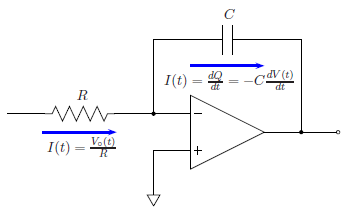
\includegraphics[width=1.5in]{7.1.2/Circuit_Diagram.png}
\caption{Experiment 7.1.2 Circuit *coppied from lab manual.}
\end{figure}\\
Components:\\
Opamp: TL071  Capacitor: 1$\mu$F  Resistor: 1k$\Omega$  \\Trim: Potentiometer: 100k$\Omega$ Resistor: 1.5k$\Omega$\\
Collect traces of the output waveform with input square wave frequencies of: 50, 100, 200, 500, 1000, 5000 Hz.
\newpage
\subsection*{7.1.3}

Integrating opamp with capacitor and extra resistor.
\begin{figure}[h]
\centering
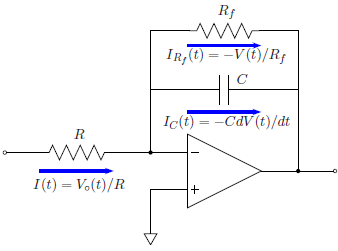
\includegraphics[width=1.5in]{7.1.3/Circuit_Diagram.png}
\caption{Experiment 7.1.3 Circuit *coppied from lab manual.}
\end{figure}\\
Components:\\
Identical to 7.1.2 however, an additional resistor Rf: 1M$\Omega$ was added.\\
Collect the same traces as 7.1.2.\\
\subsection*{7.1.4}
Circuit and components identical to 7.1.3.\\
Use the response spectrum to obtain amplitude and phase plot.\\
\newpage
\subsection*{7.2.1}
Differentiating opamp with capacitor.
\begin{figure}[h]
\centering
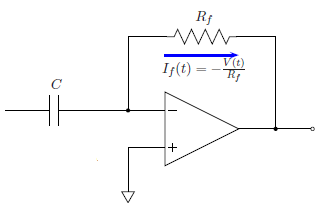
\includegraphics[width=1.5in]{7.2.1/Circuit_Diagram.png}
\caption{Experiment 7.2.1 Circuit *coppied from lab manual.}
\end{figure}\\
Components:\\
Identical to 7.1.2.\\
Collect traces similar to 7.1.2.
\subsection*{7.2.2}
Differentiating opamp frequency analysis.
Circuit and components identical to 7.2.1.\\
Use the response spectrum to obtain amplitude and phase plot.
\newpage
\subsection*{7.3.1}
Band-pass filter.
\begin{figure}[h]
\centering
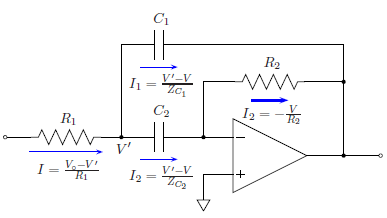
\includegraphics[width=1.5in]{7.3.1/Circuit_Diagram.png}
\caption{Experiment 7.3.1 Circuit *coppied from lab manual.}
\end{figure}\\
Components:\\
Opamp: TL071 R1: 2k$\Omega$  R2: 200k$\Omega$  C1, C2: 20pF\\
Collect traces similar to 7.1.2.

\section*{Results}

\subsection*{7.1.2}
Trace:
\begin{figure}[h]
\centering
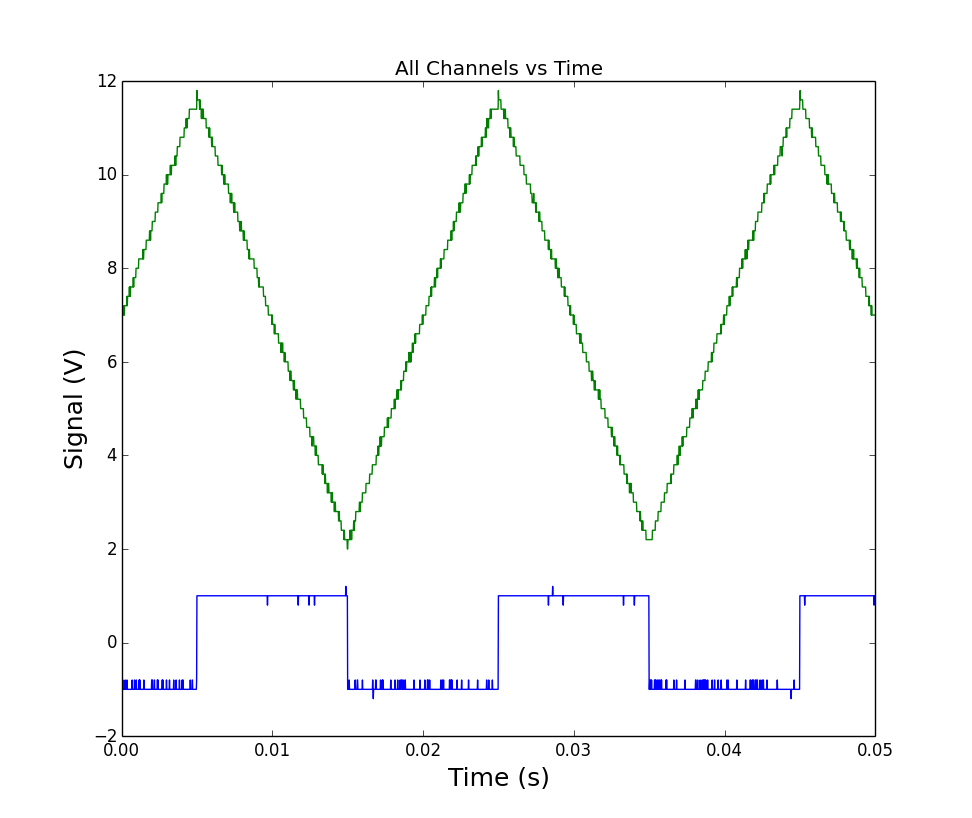
\includegraphics[width=1.5in]{7.1.2/lab7_1_2_50hz_ch1_ch2.png}
\caption{Experiment 7.1.2 50hz input (blue) and output(green)}
\end{figure}\\
Traces collected for all requested frequencies.  Traces and data available if needed, more would be added in final draft.

\subsection*{7.1.3}
Trace:
\begin{figure}[h]
\centering
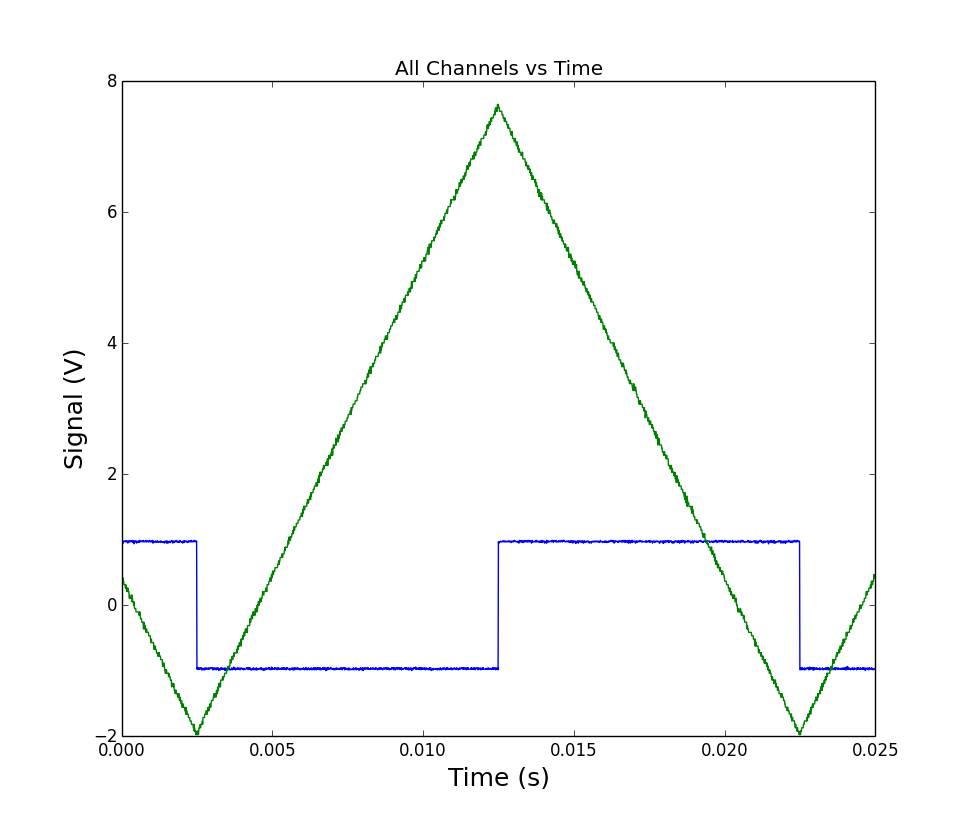
\includegraphics[width=1.5in]{7.1.3/lab7_1_3_50hz_ch1_ch2.png}
\caption{Experiment 7.1.3 50hz input(blue) and output(green)}
\end{figure}\\
Traces collected for all requested frequencies.  Traces and data available if needed, more would be added in final draft.

\subsection*{7.1.4}
Traces:
\begin{figure}[h]
\centering
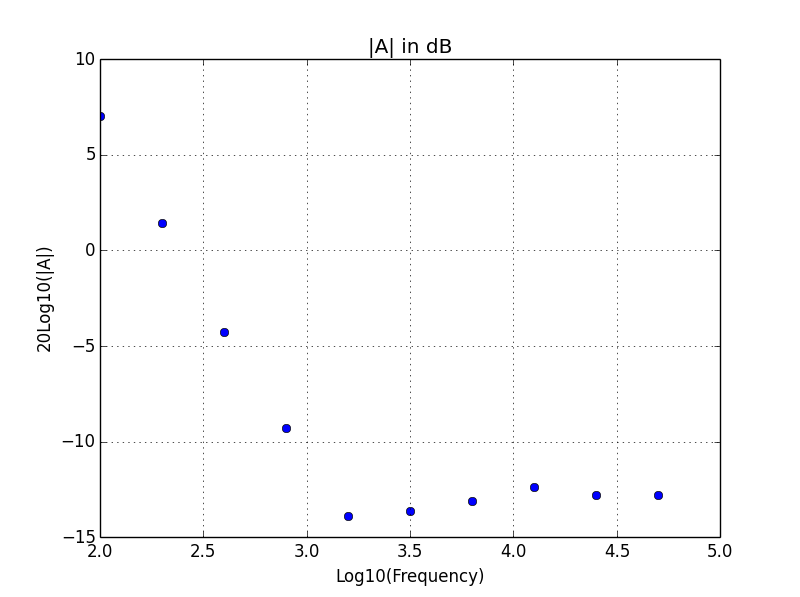
\includegraphics[width=1.5in]{7.1.4/lab7_1_4_Amplitude.png}
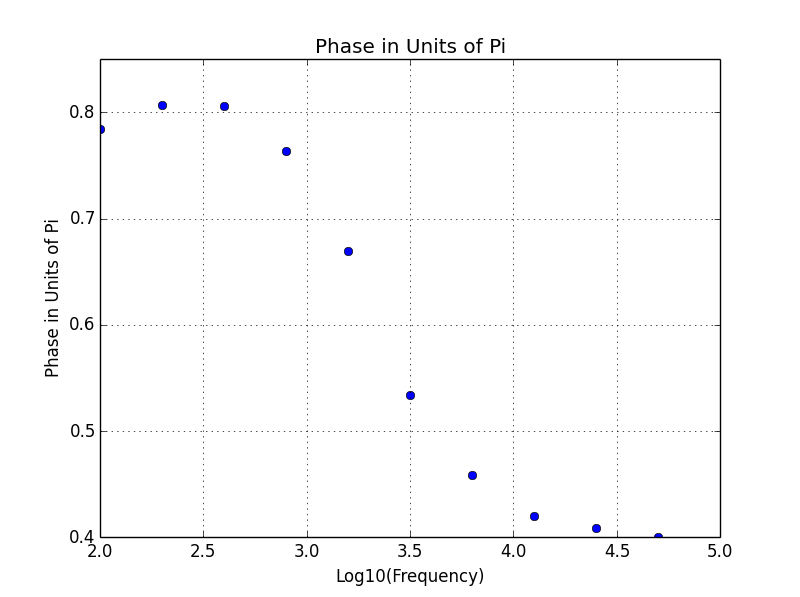
\includegraphics[width=1.5in]{7.1.4/lab7_1_4_Phase.png}
\caption{Experiment 7.1.4 Amplitude(left) and Phase(right)}
\end{figure}\\
Data available upon request.
\newpage
\subsection*{7.2.1}
Trace:
\begin{figure}[h]
\centering
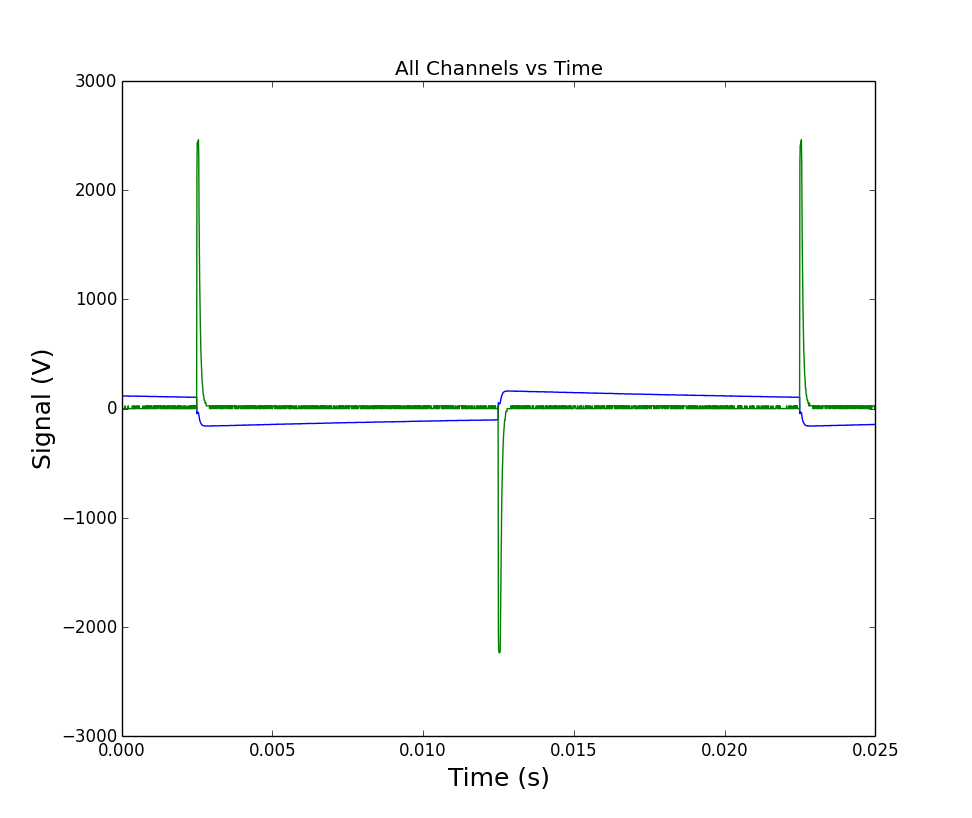
\includegraphics[width=1.5in]{7.2.1/lab7_2_1_50hz_ch1_ch2.png}
\caption{Experiment 7.2.1 50hz input(blue) and output(green)}
\end{figure}\\
All requested frequencies and data available upon request.

\subsection*{7.2.2}
Traces:
\begin{figure}[h]
\centering
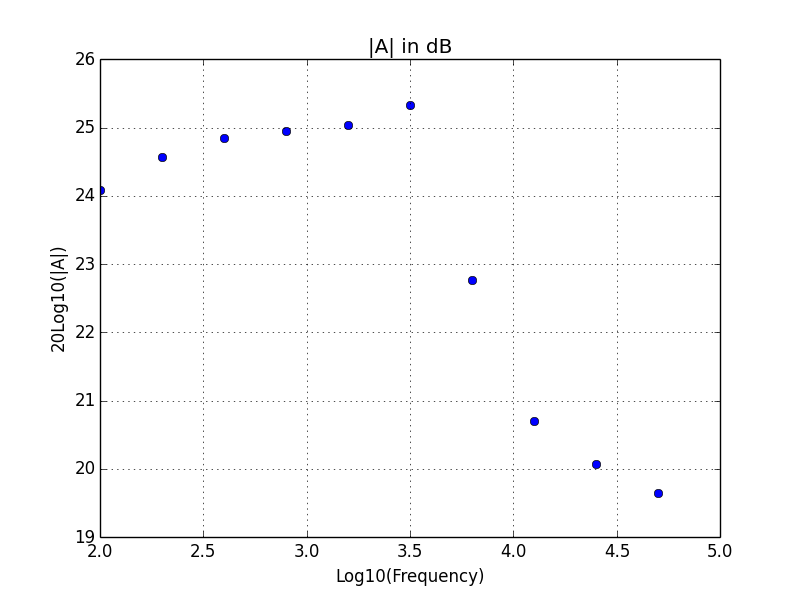
\includegraphics[width=1.5in]{7.2.2/lab7_2_2_Amplitude.png}
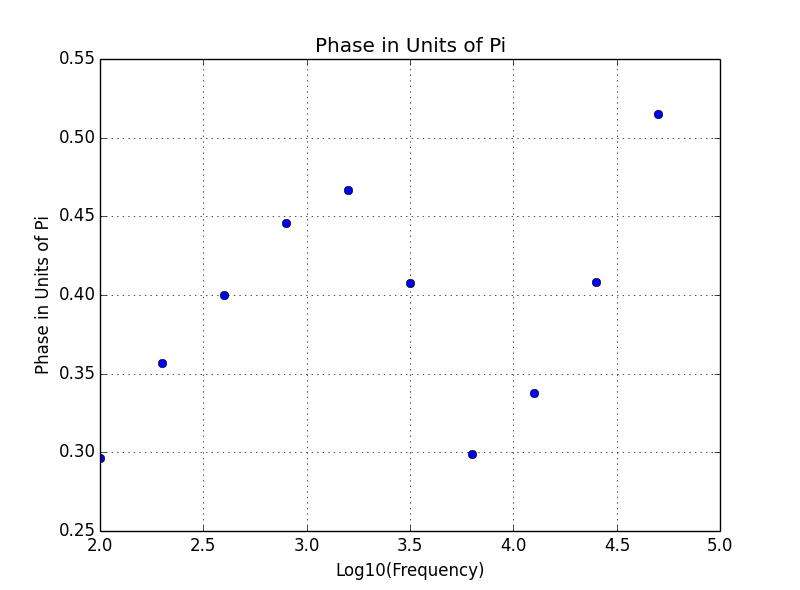
\includegraphics[width=1.5in]{7.2.2/lab7_2_2_Phase.png}
\caption{Experiment 7.2.2 Amplitude(left) and Phase(right)}
\end{figure}\\
Data missing from file.

\newpage
\subsection*{7.3.1}
Trace:
\begin{figure}[h]
\centering
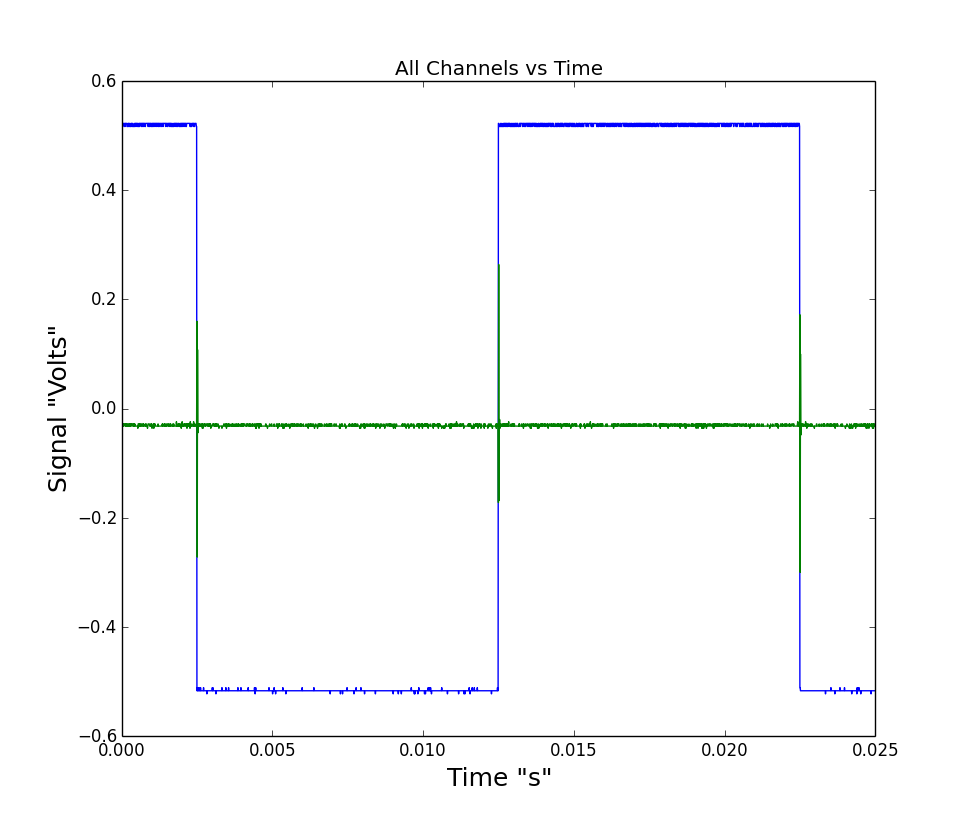
\includegraphics[width=1.5in]{7.3.1/lab7_3_1_50hz_ch1_ch2.png}
\caption{Experiment 7.3.1 50hz input(blue) and output(green)}
\end{figure}\\
All requested frequencies and data available upon request.

\section*{Error Analysis}
Need to document the function generator and oscilloscope error stats.\\
The resistors used have a 5\% error in their values.

The human element of error is in the circuit setup and possible crossed wires.  The choice of using gator clips for some connections adds another source of error.  Try to eliminate the use of gators in the future.

\section*{Discussion}
All of the experiments are to be compared to passive circuits built in ph 411.\\
The main problem with this lab initially was setting up the circuit.  The first opamp used was dead and it took some time to troubleshoot it.


\section*{Conclusion}
Data was obtained for the opamp circuits and can be compared to the passive circuits obtained last term.
\end{document}
